\documentclass[11pt]{standalone}
\usepackage[usenames]{color} %used for font color
\usepackage{amssymb} %maths
\usepackage{amsmath} %maths

\usepackage[no-math]{fontspec}
\usepackage{unicode-math}
\setmainfont{Lato}
\setmathfont{Stix Two Math}

\usepackage{pgf,xcolor}
\definecolor{itwm_blue_04}{HTML}{005A94}
\definecolor{itwm_red}{HTML}{C00000}
\definecolor{itwm_yellow}{HTML}{FFEC7F}

\usepackage{tikz}
\usetikzlibrary{shapes.misc, shadows, decorations, arrows}
\usetikzlibrary{backgrounds}
\usetikzlibrary{calc}
\usepackage{pgfplots}
\pgfplotsset{compat=newest}
\usepgfplotslibrary{fillbetween}
\usepackage{tikzpagenodes}
\usetikzlibrary{patterns}

% 0,1 x 1,2
\begin{document}
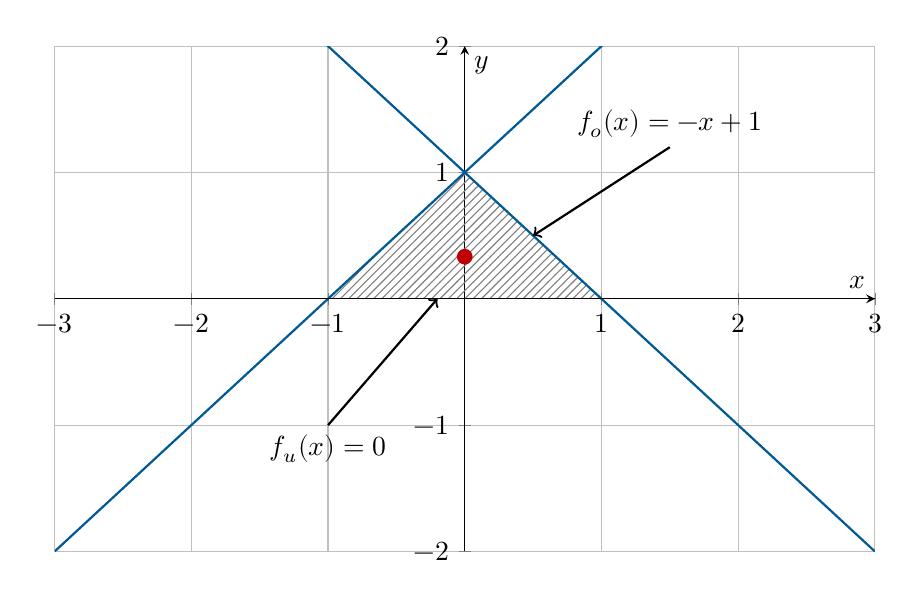
\begin{tikzpicture}
\begin{axis}[
    domain=-3:3,
    axis lines = center,
    xlabel = {$x$},
    ylabel = {$y$},
    height=8cm, width=12cm, 
    xmin=-3, xmax=3, ymin=-2, ymax=2, 
    xtick={-3, -2,...,3},
    ytick={-2, -1,...,2},
    grid = both
]
\addplot[draw=itwm_blue_04, samples=300, thick, name path=f]{-x+1};
\addplot[draw=itwm_blue_04, samples=300, thick, name path=g]{x+1};
\addplot[name path=a]{0};
%\node[fill, itwm_blue_04, circle,inner sep=-2] at (-3,4) {};
%\node[fill, itwm_blue_04, circle,inner sep=-2] at (2,-1) {};
\node at (-1.5, 4.25) {$f_o(x)=-x+1$};

\addplot [pattern=north east lines, pattern color=gray] fill between [of = f and a, soft clip={domain=0:1}];
\addplot [pattern=north east lines, pattern color=gray] fill between [of = g and a, soft clip={domain=-1:0}];
%\node at (1.25, 4.5) {Schwerpunkt};
\node[fill, itwm_red, circle,inner sep=-2] at (0,1/3) {};
\draw [->, thick] (-1, -1) -- (-0.2,0) {};
\node [below] at (-1, -1) {$f_u(x)=0$};
\draw [->, thick] (1.5, 1.2) -- (0.5,0.5) {};
\node [above] at (1.5, 1.2) {$f_o(x)=-x+1$};

\end{axis}
\end{tikzpicture}
\end{document}